\chapter{Resultados experimentales.}
% ----------------------

\label{C:Resultados_experimentales.}

\section{Resultados para el modo de tensión}
En esta sección se evalúa el rendimiento de la fuente en su primer modo de operación, donde se configura el nivel de tensión de salida deseado y se establece una corriente máxima de salida. Si la corriente supera el valor límite, la fuente ajustará automáticamente la tensión de salida para evitar exceder el flujo de corriente permitido. \par  
Se realizaron varias pruebas para analizar el comportamiento de la fuente bajo distintas condiciones operativas. Los resultados obtenidos permiten delimitar las características de funcionamiento del sistema en escenarios típicos de operación. \par 
\subsection{Valor de carga fijo al energizar}
En esta subsección se presentan los resultados obtenidos al energizar la fuente con una carga fija previamente conectada. El objetivo de esta prueba es observar el comportamiento inicial de la tensión de salida al aplicar la carga y verificar que el sistema mantiene el nivel de tensión configurado sin exceder los límites de corriente establecidos.\par
En las Figuras \ref{F:Energizacion15} y \ref{F:Energizacion25} se muestran los resultados obtenidos utilizando una carga resistiva de aproximadamente $30\Omega$. La prueba se realizó configurando la fuente en 15V y 25V respectivamente.
\begin{figure}[htbp]
    \centering
    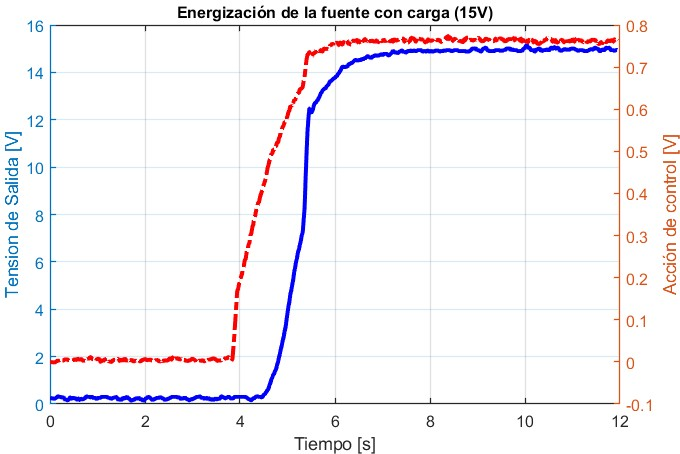
\includegraphics[width=0.8\textwidth]{./imagenes/Energizacion15.jpg}
    \caption{Respuesta obtenida al energizar la fuente configurada en 15V con una carga conectada.}
    \label{F:Energizacion15}
\end{figure}

\begin{figure}[htbp]
    \centering
    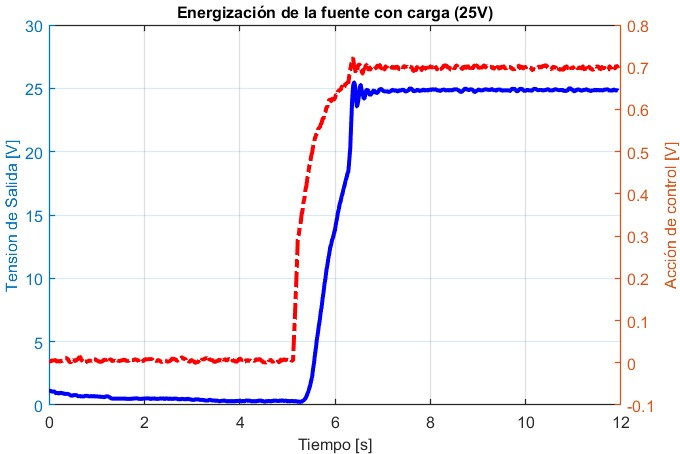
\includegraphics[width=0.8\textwidth]{./imagenes/Energizacion25.jpg}
    \caption{Respuesta obtenida al energizar la fuente configurada en 25V con una carga conectada.}
    \label{F:Energizacion25}
\end{figure}\par 
Los gráficos muestran una respuesta transitoria satisfactoria, alcanzando el valor de referencia con un tiempo de asentamiento cercano a un segundo. Además, no se observa un sobrepaso significativo, lo cual indica que la fuente opera de manera estable bajo las condiciones evaluadas.\par 

\subsection{Conexión de carga}
En esta subsección se presentan los resultados obtenidos al conectar una carga con la fuente ya energizada.  El objetivo de esta prueba es evaluar la capacidad del sistema para ajustar rápidamente la tensión de salida al pasar de una condición sin carga (vacío) a una con carga aplicada. \par
A continuación, se muestran las Figuras \ref{F:Conexion15} y \ref{F:Conexion25}, donde se observan las respuestas del sistema para dos valores de tensión de salida diferentes: 15V y 25V.\par 

\begin{figure}[htbp]
    \centering
    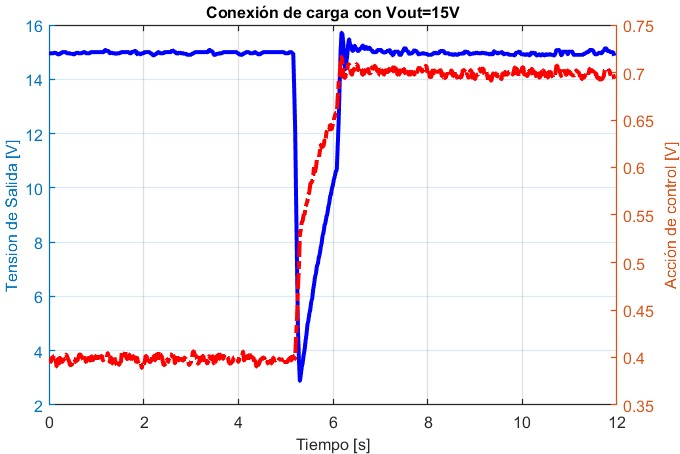
\includegraphics[width=0.8\textwidth]{./imagenes/Conexion2.jpg}
    \caption{Respuesta obtenida al pasar del estado de vacío al de carga con Vout=15V.}
    \label{F:Conexion15}
\end{figure}\par 

\begin{figure}[htbp]
    \centering
    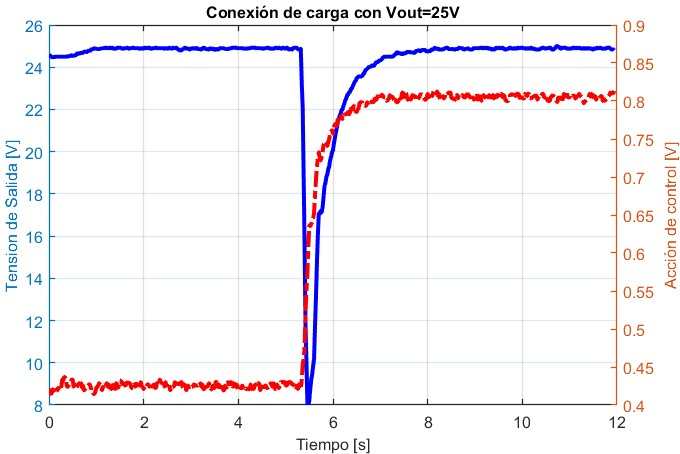
\includegraphics[width=0.8\textwidth]{./imagenes/Conexion1.jpg}
    \caption{Respuesta obtenida al pasar del estado de vacío al de carga con Vout=25V.}
    \label{F:Conexion25}
\end{figure}\par 

Los gráficos muestran una rápida respuesta del algoritmo de control, ajustando la acción de control para mantener la tensión de salida en el valor deseado. En el caso de la prueba con 15V, se observa un ligero sobrepaso, mientras que en la prueba con 25V no hay sobrepaso apreciable. Esta diferencia podría deberse al uso de ganancias más pequeñas en el rango de voltajes más altos. Aun así, en ambos casos, la respuesta es satisfactoria y dentro de los márgenes aceptables para un funcionamiento estable. \par


\subsection{Desconexión de carga}
En esta subsección se analiza el comportamiento de la fuente al desconectar una carga mientras está en funcionamiento. La prueba tiene como objetivo observar cómo responde la fuente ante una desconexión repentina y si es capaz de estabilizar la tensión de salida sin generar sobrecargas o picos no deseados.\par
Las Figuras \ref{F:Desconexion15} y \ref{F:Desconexion25} muestran los resultados obtenidos al pasar de un estado estacionario con carga conectada a una condición de vacío, es decir, sin carga. A continuación, se analiza el desempeño del sistema en cada caso.\par 
\begin{figure}[htbp]
    \centering
    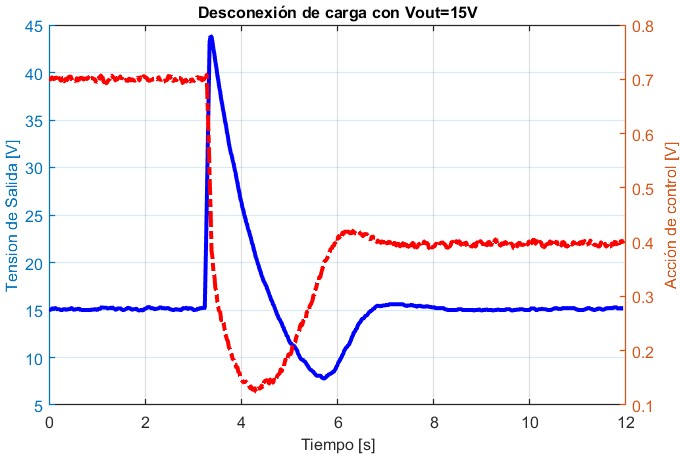
\includegraphics[width=0.8\textwidth]{./imagenes/Desconexion1.jpg}
    \caption{Respuesta obtenida al pasar del estado de carga al de vacío con Vout=15V.}
    \label{F:Desconexion15}
\end{figure}\par 
\begin{figure}[htbp]
    \centering
    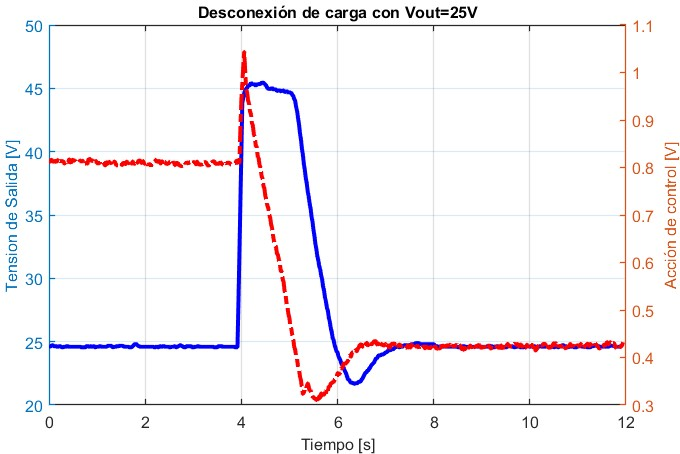
\includegraphics[width=0.8\textwidth]{./imagenes/Desconexion2.jpg}
    \caption{Respuesta obtenida al pasar del estado de carga al de vacío con Vout=25V.}
    \label{F:Desconexion25}
\end{figure}\par 
De los gráficos, se observa que la tensión de salida se incrementa bruscamente tras la desconexión de la carga, alcanzando valores cercanos a los 45V. Esto ocurre a pesar de que la acción de control disminuye rápidamente, lo que indica que, en condición de vacío, sin una carga que consuma la corriente, esta se acumula en el capacitor de salida, provocando el abrupto aumento en la tensión. \par
En el caso de la prueba con 25V, se aprecia una sobretensión de mayor duración en comparación con la prueba de 15V. Ante estas condiciones, se considera necesario añadir una lógica de desacoplamiento de la carga para prevenir que, durante un transitorio, la reconexión de una carga se someta a un valor de tensión superior al esperado. Esta medida es fundamental para evitar posibles daños en los equipos conectados. \par 

\subsection{Prueba con motor de 12 V}
En este apartado se presentan los resultados de las pruebas realizadas al conectar un motor de 12 V a la fuente de alimentación. El objetivo es analizar el comportamiento de la fuente cuando opera con una carga inductiva, así como su capacidad para manejar los picos de corriente generados durante el arranque del motor. \par 
La Figura \ref{F:Motor12} muestra el comportamiento de la tensión de salida cuando se conecta este tipo de carga. Se observa un \textit{ripple} considerable en torno al voltaje de referencia, lo que indica fluctuaciones en la salida mientras el motor está en operación. En esta prueba, el motor se encontraba sin carga mecánica adicional. \par 
\begin{figure}[htbp]
    \centering
    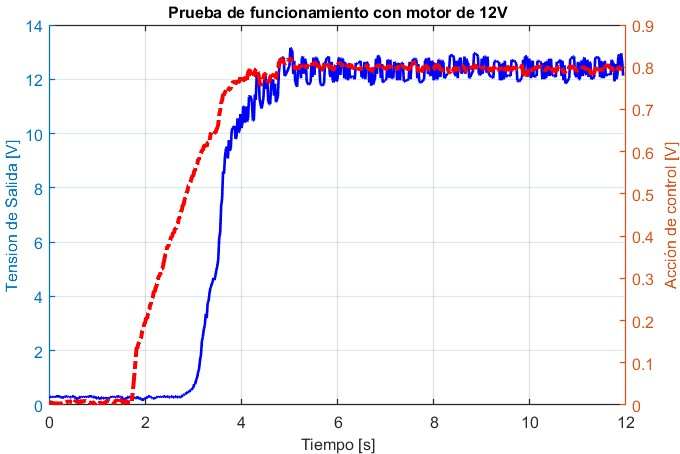
\includegraphics[width=0.8\textwidth]{./imagenes/Motor2.jpg}
    \caption{Prueba de funcionamiento con motor de 12V.}
    \label{F:Motor12}
\end{figure}\par 
El ripple observado sugiere que la fuente podría estar reaccionando a los transitorios causados por la naturaleza inductiva del motor. Es importante mencionar que este tipo de cargas pueden generar corrientes de retorno que podrían afectar la estabilidad de la fuente. \par 

\subsection{Protección por sobrecorriente}
En esta subsección se presentan los resultados de la prueba de protección por sobrecorriente. Para realizar la prueba, se incrementó gradualmente la demanda de corriente hasta superar el límite configurado, lo que activó el mecanismo de protección de la fuente. Este mecanismo reduce la tensión de salida para evitar que la corriente sobrepase el valor máximo establecido. El objetivo es verificar la efectividad del sistema de protección y la estabilidad de su respuesta en condiciones de sobrecarga. \par 
En la Figura \ref{F:Pcorriente1} se observa cómo la fuente disminuye el voltaje de salida cuando la corriente alcanza el valor límite de 1A. Durante la prueba, se realizó un barrido gradual variando los valores de resistencia de la carga, y la respuesta del sistema fue satisfactoria. Sin embargo, se sugiere realizar un ajuste fino en el acondicionador de señal de corriente para optimizar aún más el control del límite.\par 
\begin{figure}[htbp]
    \centering
    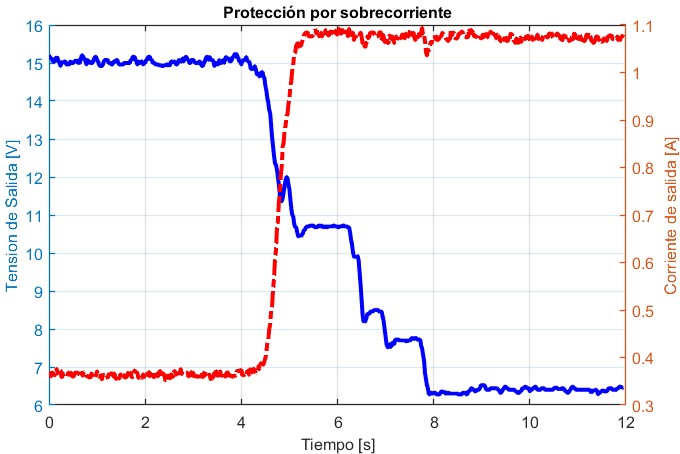
\includegraphics[width=0.8\textwidth]{./imagenes/MedicionConPuntaCorriente_proteccion.jpg}
    \caption{Respuesta obtenida de la protección por sobrecorriente.}
    \label{F:Pcorriente1}
\end{figure}\par 
La Figura \ref{F:Pcorriente2} muestra una situación similar, pero en este caso se conectó abruptamente una carga de $8,2\Omega$ en paralelo a una de $30\Omega$. A pesar de la variación brusca en la demanda de corriente, la respuesta de la fuente fue rápida y adecuada.\par 

\begin{figure}[htbp]
    \centering
    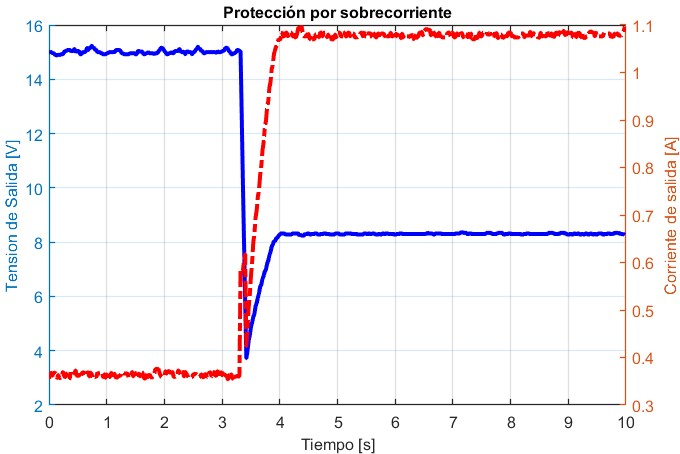
\includegraphics[width=0.8\textwidth]{./imagenes/MedicionConPuntaCorriente_proteccionRapida.jpg}
    \caption{Respuesta obtenida de la protección por sobrecorriente ante la conexión abrupta de una carga.}
    \label{F:Pcorriente2}
\end{figure}\par 

\section{Resultados para el modo de corriente} \label{S:subseccion de corriente}
Este segundo modo de operación implementa un lazo de control que regula la corriente de salida. El usuario especifica el valor de corriente deseado, y la tensión de salida de la fuente se ajusta automáticamente para mantener ese flujo de corriente. Cabe destacar que es importante mantener la carga conectada antes de energizar la salida. Si la carga está desconectada o es demasiado pequeña, el lazo de control no logrará alcanzar su referencia, lo que incrementará su acción integral. Esto resulta en una mayor tensión aplicada a la base de los transistores, pudiendo llevar la tensión de salida a niveles cercanos a $43V$. \par 
Para las pruebas, se utilizó una carga resistiva variable, configurando la corriente en $1A$ para observar el comportamiento transitorio del algoritmo de control. Los resultados obtenidos se muestran en la Figura \ref{F:Lcorriente1} .
\begin{figure}[htbp]
    \centering
    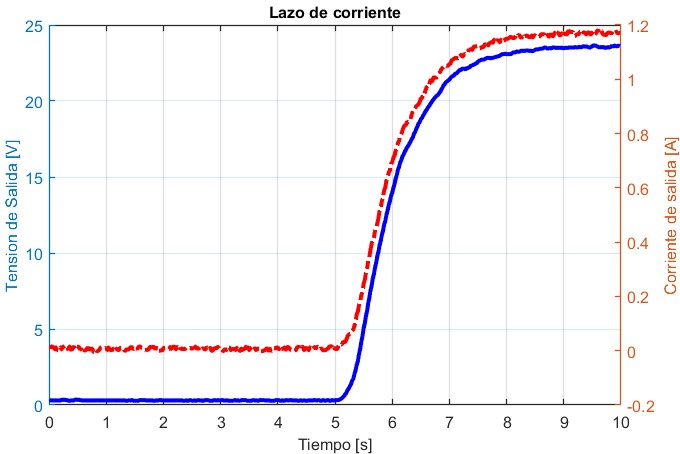
\includegraphics[width=0.8\textwidth]{./imagenes/LazoCorriente.jpg}
    \caption{Respuesta obtenida del modo corriente para una referencia de 1A.}
    \label{F:Lcorriente1}
\end{figure} \par 
Las gráficas muestran una respuesta sobreamortiguada, con un tiempo de asentamiento cercano a los dos segundos. Aunque la respuesta es algo lenta, es adecuada para evitar sobrepasos que podrían dañar los equipos conectados a la salida. Se denota que se requiere un ajuste fino del preset de la etapa acondicionadora de la señal de corriente. \par

\section{Resultados para el modo rampa}
Se realizaron ensayos para verificar el correcto funcionamiento del tercer modo de operación, que corresponde a un perfil de rampa. En este modo, el valor de referencia de tensión se incrementa gradualmente hasta alcanzar el valor fijado por el usuario en un tiempo determinado. \par 
A continuación se presentan las Figuras \ref{F:Rampa24_16} y \ref{F:Rampa24_30}, donde se puede observar la respuesta obtenida en los ensayos. Los experimentos se realizaron utilizando una carga resistiva inferior a $100\Omega$. \par
\begin{figure}[htbp]
    \centering
    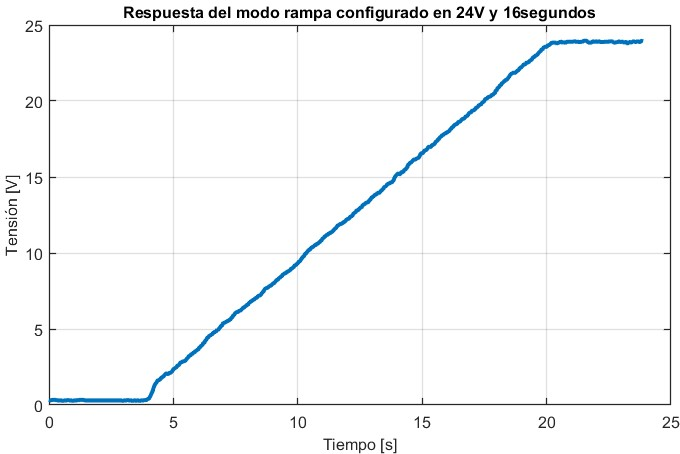
\includegraphics[width=0.8\textwidth]{./imagenes/Rampa_24_16.jpg}
    \caption{Respuesta obtenida del modo rampa para una configuración de 24 V y 16segundos.}
    \label{F:Rampa24_16}
\end{figure}
\begin{figure}[htbp]
    \centering
    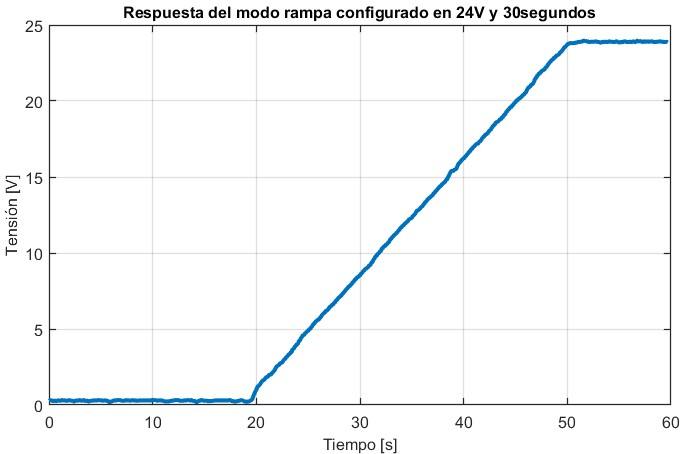
\includegraphics[width=0.8\textwidth]{./imagenes/Rampa_24_30.jpg}
    \caption{Respuesta obtenida del modo rampa para una configuración de 24 V y 30segundos.}
    \label{F:Rampa24_30}
\end{figure}\par 
En las gráficas se puede apreciar un crecimiento lineal de la tensión conforme al tiempo establecido. Se observa un mayor incremento en los primeros instantes de la rampa, lo cual es atribuible a la estrategia de control implementada. Sin embargo, este efecto es insignificante y no compromete el correcto funcionamiento del sistema.\par 

\section{Análisis de la tensión de entrada}
Para determinar el rango de operación de la fuente de alimentación, se analizó el comportamiento de la tensión de entrada rectificada antes del regulador basado en BJT. Este análisis permite evaluar la estabilidad y el margen de operación de los transistores en la zona activa, incluso bajo condiciones de carga variables. \par

Se presentan dos condiciones principales para observar el comportamiento de la tensión de entrada. En primer lugar, se evaluó el funcionamiento en una condición de baja corriente, en torno a 200 mA, como se muestra en la Figura \ref{F:Tension_entrada_12}.En esta figura, se observa que cuando la fuente está desactivada, la tensión rectificada se mantiene cerca de 46 V. Sin embargo, al habilitar la salida y establecer un nivel de tensión dado, la tensión de entrada desciende hasta aproximadamente 34 V. Este descenso es aceptable y evidencia un margen de operación adecuado para los transistores, asegurando su funcionamiento en la zona activa incluso si se incrementa la tensión de salida hasta 30 V. \par

\begin{figure}[htbp]
    \centering
    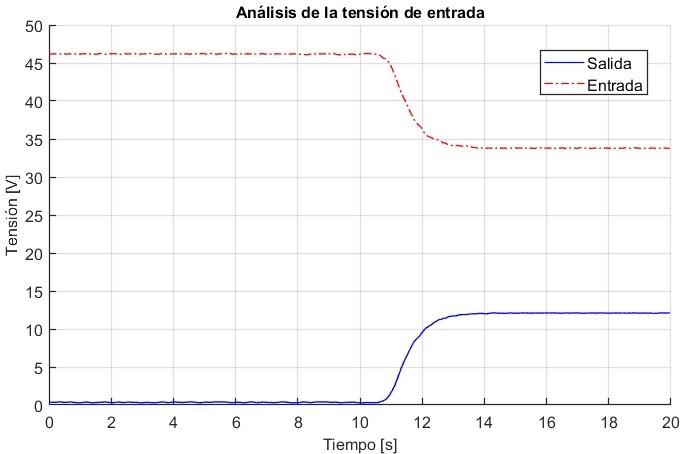
\includegraphics[width=0.8\textwidth]{./imagenes/Tension_12.jpg}
    \caption{Análisis de la tensión de entrada frente a un punto de operación normal.}
    \label{F:Tension_entrada_12}
\end{figure}\par

La segunda condición analizada corresponde a la corriente de salida máxima, en la que la fuente suministra aproximadamente 3 A. La Figura \ref{F:Vrec_Isal} muestra el análisis de la tensión de entrada bajo esta carga nominal. Al exigir esta corriente, se observa que la tensión de entrada vuelve a caer, similar al caso anterior, pero se mantiene por encima de 34 V. Este resultado confirma que, incluso en condiciones de máxima demanda de corriente, los transistores continúan operando dentro de la zona activa, manteniendo así el margen necesario para una regulación estable. \par

\begin{figure}[htbp]
    \centering
    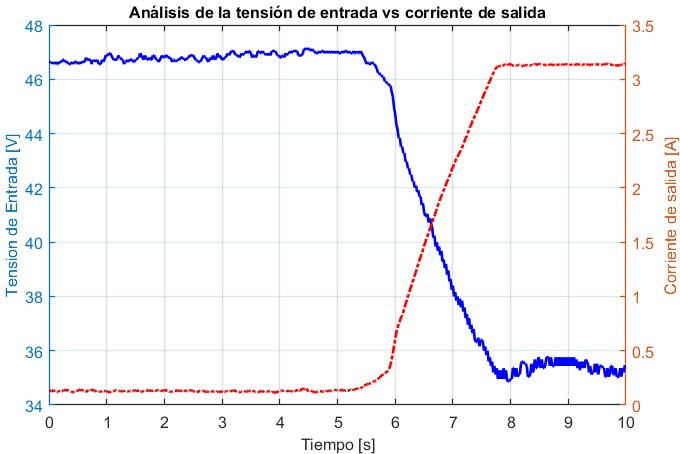
\includegraphics[width=0.8\textwidth]{./imagenes/Vrec_Isal.jpg}
    \caption{Análisis de la tensión de entrada frente a una condición de carga nominal.}
    \label{F:Vrec_Isal}
\end{figure}\par 

Finalmente, se analizó el rizado en la tensión de entrada para esta última condición de carga máxima. Para capturar el rizado, se configuró el osciloscopio en modo de acoplamiento de corriente alterna (CA), permitiendo medir exclusivamente el componente de riple. La Figura \ref{F:ripple} muestra los resultados obtenidos, donde se observa un rizado de aproximadamente 2 V pico a pico con una frecuencia cercana a 100 Hz, correspondiente al rectificador de onda completa. Estos valores de rizado son aceptables, confirmando el correcto funcionamiento de la fuente dentro del rango especificado en los objetivos del diseño.

\begin{figure}[htbp]
    \centering
    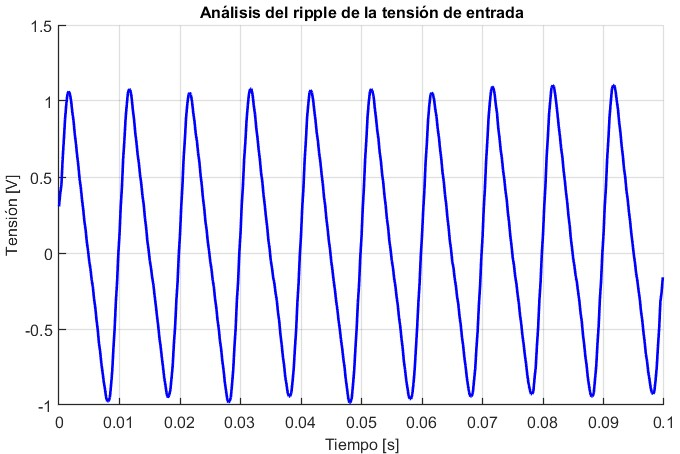
\includegraphics[width=0.8\textwidth]{./imagenes/ripple.jpg}
    \caption{Análisis de la tensión de entrada frente a una condición de carga nominal.}
    \label{F:ripple}
\end{figure}\par 


